\documentclass[12pt, titlepage]{article}
\usepackage{fancyhdr}
\usepackage{tikz}
\usetikzlibrary{patterns}
\usepackage{caption}

\pagestyle{fancy}
\fancyhead[L]{Fluid Simulation}
\fancyhead[R]{Documentation}

\usepackage{amsmath}
\begin{document}

\pagestyle{fancy}

\title{Fluid Simulation Documentation}
\author{Nagy Balázs EIO1RQ}
\date{\today}
\maketitle

\tableofcontents

\pagebreak

\section{Introduction}

This project and the subsequent program code has been produced for the purposes of completing the Summer Internship at the University of Miskolc. The aim of the program is to simulate fluid flow in a limited region of space along with handling changes in pressure and in the velocity flow field. For the sake of simplicity the fluid is treated as incompressible and is assumed to be of low velocity (below 100$\frac{m}{s}$). Furthermore since total accuracy is not the main goal physical phenomena such as the boundary layer, no slip condition, surface tension and any effects relating to Reynolds numbers are ignored.

\section{Initial approach}

\subsection{Eulerian vs Lagrangian Coordinates}
In fluid mechanics the continuity equation assumes that fluid continoues everywhere, however since computers are limited by memory and other physical aspects the need for discretization of such quantities is imperative. The solution comes in two different ways: we have to option of using either Eulerian or Lagrangian Coorinates in order to discretize values and calculate local changes and subsequently the change in the entirety of the fluid.

Both of these approaches have their respective advantages and drawbacks.

\begin{figure}[b]
\centering
\begin{minipage}{.5\textwidth}
  \centering
  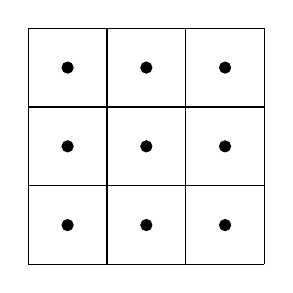
\begin{tikzpicture}
	\draw[step=1cm] (0, 0) grid (3cm, 3cm);
	\foreach \x in {0.5, 1.5, 2.5}
		\foreach \y in {0.5, 1.5, 2.5}
		{
			\filldraw (\x, \y) circle (2pt);
		}
\end{tikzpicture}
  \captionof{figure}{Grid based}
  \label{fig:test1}
\end{minipage}%
\begin{minipage}{.5\textwidth}
  \centering
  \begin{tikzpicture}
	\draw (0, 0) .. controls (1, 1) and (1, -1.4) .. (3, 1);
	\draw (0, -1) .. controls (1, 0) and (1, -2.4) .. (3, 0);
	\draw (0, -2) .. controls (1, -1) and (1, -3.4) .. (3, -1);
\end{tikzpicture}
  \captionof{figure}{Particle based}
  \label{fig:test2}
\end{minipage}
\end{figure}


The \textbf{Eulerian} way partitions the space into a grid and treats each cell as a localized region containing average data. As the size of the grid increases these localized cells become smaller, thus improving accuracy since the approximations of local values will be more accurate as well.

On the other hand, the using \textbf{Lagrangian} Coordinates we instead simulate individual particles and calculate their path and behavior while interacting with the environment.
At large scales this becomes more complex than the previous approach

\subsection{Restrictions}
The assumption of fluid \textbf{incompressibility} allows us to make use of the Navier-Stokes equations, which describe the flow of incompressible fluids, thus greatly simplífying the calculations needed.
Furthermore only \textbf{homogenous materials} are used; mixing of different fluids is not part of the simnulation.
\textbf{Viscosity} is not given as a property of the fluid, but rather implied by the use of limiting the diffusion rate.


\section{Pressure Field}

\subsection{Simple heuristics}

The equalization of pressure across the given region is almost instantaneous when adding pressure sources to it. For a simple heuristic simulation the following approach can be used:
\[ 
x_{i, j} = \frac{x_{i, j} + x_{i+1, j} + x_{i-1, j} + x_{i, j+1} + x_{i, j-1}}{5}
\]

This is adequate hydrostatic problems, since there is no movement in the fluid.

\subsection{Problems}
For small areas, specifically the localozed region defined by the cells being averaged, this works, however since this is effectively an averaging kernel that goes through the entire grid there are bound to be losses in the global domain. 

\bigskip

Although this results in pressure losses and does not adhere to the conservation of energy we can still leverage it by stating that the global region of interest, the entire area being simulated, is not bounded nor constrained by anything, as if being a localized region of a greater system itself. Much like if one were to examine a volume of 1 $m^3$ of water in the ocean. If this system is large enough than no further problems will be caused by this discrepancy.

\bigskip

As mentioned in the restricions there are many physical effects not accounted for, especially at the edges and in the corners of the grid, however since the distribution of pressure is defined as an average of a given cell and its neighbours' these cases must be handeled regardless.

Possible solutions are to limit the space that the kernel iterates through and leave a 1 cell thick \textit{border} on all sides, and or change the size (consequently the shape) of the kernel making it a $3x3$ square, which would get eliminate the problems caused by the corners.

\subsection{Diffusion}

When the velocity flow field is taken into account the issue of pressure distribution becomes much harder. This change with respect to time can be described by differentioal equations, but these would introduce much more calculations and solving for each individual cell is costly.

\begin{center}
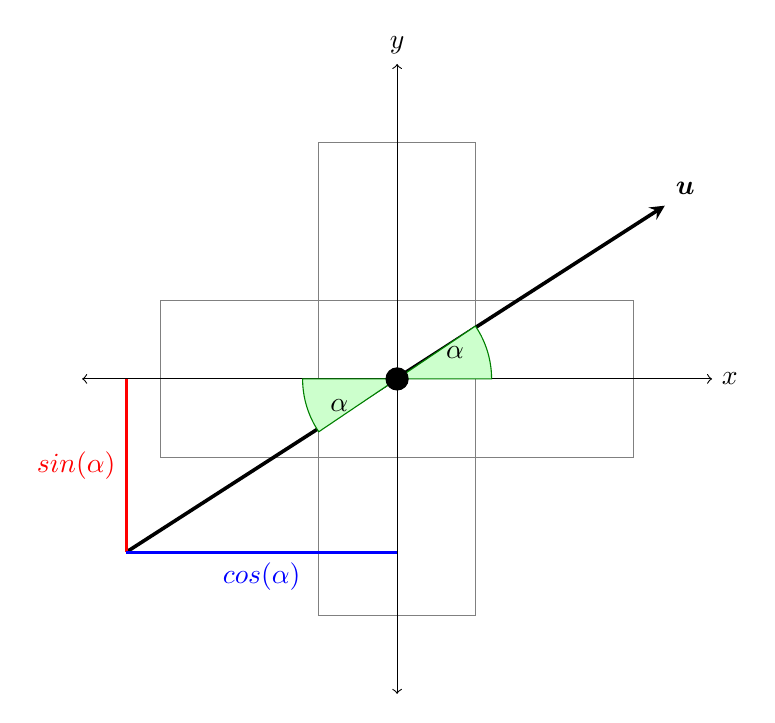
\begin{tikzpicture}[scale=2]
	%\filldraw[lightgray] (0, 0) rectangle (1, 1);
	\draw[gray] (0, 0)	rectangle (1, 1);
	\draw[gray] (0, 1)	rectangle (1, 2);
	\draw[gray] (-1, 0) rectangle (0, 1);
	\draw[gray] (0, -1) rectangle (1, 0);
	\draw[gray] (1, 0)	rectangle (2, 1);

	\draw[<->] (-1.5, 0.5) -- (2.5, 0.5) node[right]{$x$};
	\draw[<->] (0.5, -1.5) -- (0.5, 2.5) node[above]{$y$};
	
	\draw[line width=1.3pt,-stealth](-1.22, -0.6)--(2.2, 1.6) node[anchor=south west]{$\boldsymbol{u}$};
	
	\draw[red,very thick] (-1.22, -0.6) -- (-1.22, 0.5) node[midway, left]{$sin(\alpha)$};
	\draw[blue,very thick] (-1.22, -0.6) -- (0.5, -0.6) node[midway, below]{$cos(\alpha)$};
	
	\filldraw[fill=green!20!white, draw=green!50!black] (0.5, 0.5) -- (1.1, 0.5) arc (0:34:0.6) -- cycle node[midway, right]{$\alpha$};
	\filldraw[fill=green!20!white, draw=green!50!black] (0.5, 0.5) -- (-0.1, 0.5) arc (180:214:0.6) -- cycle node[midway, left]{$\alpha$};
	
	\filldraw (0.5, 0.5) circle (2pt);
\end{tikzpicture}
\end{center}

So instead we alter the previous calculations and now include information about the vector field as well. The flow in each localized region is described by a single vector, whose direction and magnitude correspond to the fluid's flow direction and speed respectively.

\bigskip

The direction of flow also determines how the pressure changes, so any alterations in the flow velocity field will cause a change in pressure distribution.
Instead of using conventional averages we use weighted averages where the weights are the distance of grids located in the path of fluid flow from the vector itself.
The \textit{closer} a vector is to a grid cell the more significantly it contributes to the change in pressure. 

These distances are the $sin(\alpha)$ and $cos(\alpha)$ in the $y$ and $x$ directions respectively. After normalizing the vector there is no need to calculate these values and we can just use the $x$ and $y$ coordinates of the subsequent unit vector.

Cells on the $x$ axis are weighted with $sin(\alpha)$ and grid cells located on the $y$ axis are multiplied by $cos(\alpha)$. The calculation is done in the following manner:

\[
	vec = \text{normalized vector at }cell_{i, j}
\]

\[
	cell_{i, j} = \begin{cases}
	vec.x \cdot cell_{i+1, j} + vec.y \cdot cell_{i, j-1}, & x > 0, y > 0 \\
	vec.x \cdot cell_{i-1, j} + (-1)\cdot vec.y \cdot cell_{i, j-1}, & x > 0, y < 0 \\
	(-1) \cdot vec.x \cdot cell_{i-1, j} + (-1) \cdot vec.y \cdot cell_{i, j+1}, & x < 0, y < 0 \\
	(-1) \cdot vec.x \cdot cell_{i-1, j} + vec.y \cdot cell_{i, j+1}, & x < 0, y > 0
	\end{cases}
\]

\section{Velocity Flow Field}



\end{document}